\documentclass[aspectratio=169]{beamer}
\usepackage[utf8]{inputenc}
\usepackage{hyperref}
\usepackage{amsmath,amsfonts,amsthm,bm}
\usepackage{color}
\usepackage{graphicx} % Allows including images
\usepackage{subcaption}
\usepackage{booktabs} % Allows the use of \toprule, \midrule and \bottomrule in tables
\usepackage{tikz}
\usepackage{color}
\usepackage{minted}
\usetikzlibrary{automata,positioning,shapes.geometric,shapes.misc,arrows}
%\usepackage{pgfplots}
\usepackage{listings}
\usepackage{courier}
\usepackage[version=4]{mhchem}
\usepackage{array}

\lstset{ %
    basicstyle=\scriptsize\ttfamily, % fonts that are used for the code
    breakatwhitespace=false,         % sets if automatic breaks should only happen at whitespace
%breaklines=true,                 % sets automatic line breaking
%captionpos=b,                    % sets the caption-position to bottom
    commentstyle=\color{gray}\textit,    % comment style
    keepspaces=true,                 % keeps spaces in text, useful for keeping indentation of code (possibly needs columns=flexible)
    keywordstyle=\color{blue},       % keyword style
    language=Python,                 % the language of the code
%otherkeywords={*,...},          % if you want to add more keywords to the set
    rulecolor=\color{black},         % if not set, the frame-color may be changed on line-breaks within not-black text (e.g. comments (green here))
    showspaces=false,                % show spaces everywhere adding particular underscores; it overrides 'showstringspaces'
    showstringspaces=false,          % underline spaces within strings only
    showtabs=false,                  % show tabs within strings adding particular underscores
    stringstyle=\color{red}, % string literal style
    tabsize=4,                       % sets default tabsize to 2 spaces
    columns=fixed                    % Using fixed column width (for e.g. nice alignment)
}

\hypersetup{
    colorlinks=true,
    linkcolor=red,
    filecolor=magenta,
    urlcolor=red,
}

\DeclareMathOperator*{\argmax}{argmax}
\DeclareMathOperator*{\argmin}{argmin}
\let \vec \mathbf

\newcommand{\classname}{NANO266}
\newcommand{\classyear}{Fall 2024}
\mode<presentation> {
    \usetheme{CambridgeUS}
    \setbeamertemplate{footline}[text line]{%
        \parbox{\linewidth}{\vspace*{-8pt}\classname\hfill\classyear\hfill\insertpagenumber}}

    %\setbeamertemplate{footline}[page number]
    \setbeamertemplate{navigation symbols}{}
}


\title[\classname Tools of the Modelling Trade]{\classname~- Quantum Mechanical Modeling of Materials and Nanostructures\\Tools of the Modelling Trade}

\author{Shyue Ping Ong}
\institute[UCSD]{University of California, San Diego\\
\medskip
}
\date{\classyear} % Date, can be changed to a custom date

\begin{document}


    \begin{frame}
        \titlepage % Print the title page as the first slide
    \end{frame}

    \begin{frame}{It is not just about QM}
        \begin{figure}
            \centering
            \centering
            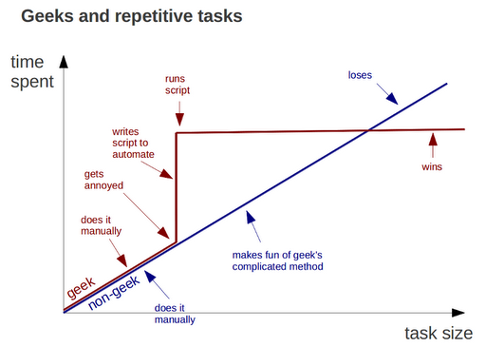
\includegraphics[width=0.6\linewidth]{lectures/figures/9_geeks.png}

        \end{figure}
    \end{frame}

    \begin{frame}{Useful unix commands}

        \begin{table}[h]
            \centering
            \begin{tabular}{l|p{12cm}}

                \textbf{Command} & \textbf{Purpose}                                                                                     \\
                \hline
                man $<$name$>$   & Display manual for command                                                                           \\
                grep             & Searches any given input files, selecting lines that match one or more patterns.                     \\
                cat              & Reads files sequentially, writing them to the standard output.                                       \\
                sed              & Reads the specified files, modifying the input as specified by a list of commands.                   \\
                tail             & Displays last part of a file.                                                                        \\
                head             & Displays start of a file.                                                                            \\
                find             & Recursively descends the directory tree, evaluating an expression in terms of each file in the tree. \\
                less             & View file in terminal.
            \end{tabular}
        \end{table}

    \end{frame}

    \begin{frame}{Unix Shells}
        Many types of Unix shell available, but broadly falls into:
        \begin{itemize}
            \item Bourne shell – de facto standard
            \item C shell – uses C-like syntax
            \item Zsh - Extended Bourne shell with many improvements, including some features of Bash, ksh, and tcsh.
        \end{itemize}

        Pick one that suits you and just set all your resources to go into that shell by default.

    \end{frame}

    \begin{frame}[fragile]{Shell scripts}
        Next level beyond just typing commands in the terminal. Writing scripts to execute sequence of commands, with some flow control where necessary.

        \inputminted{bash}{code/9_unix_for.sh}
    \end{frame}

    \begin{frame}{Flow Control}
        Specification of the order in which the individual statements, instructions or function calls of an imperative program are executed or evaluated.

        Two broad types:
        \begin{itemize}
            \item Conditional: if-else, case-switch, etc.
            \item Loops: for, while, etc.
        \end{itemize}

    \end{frame}

    \begin{frame}{Pros and Cons of Shell Scripts}
        \begin{columns}
            \column{0.7\textwidth}
            Pros
            \begin{itemize}
                \item Ubiquitous
                \item Quick and dirty
                \item Useful for short programs / scripts with a little bit of flow control.
            \end{itemize}

            Cons

            \begin{itemize}
                \item Very error-prone, especially with more complex programs.
                \item Doing even simple math is ugly (don’t even bother trying to do matrix math or anything more complex).
                \item Difficult to extend and build on.
            \end{itemize}

            \column{0.3\textwidth}

            \inputminted{bash}{code/9_expr.sh}

        \end{columns}

    \end{frame}

    \begin{frame}{Beyond Shell Scripts}
        \begin{figure}
            \centering
            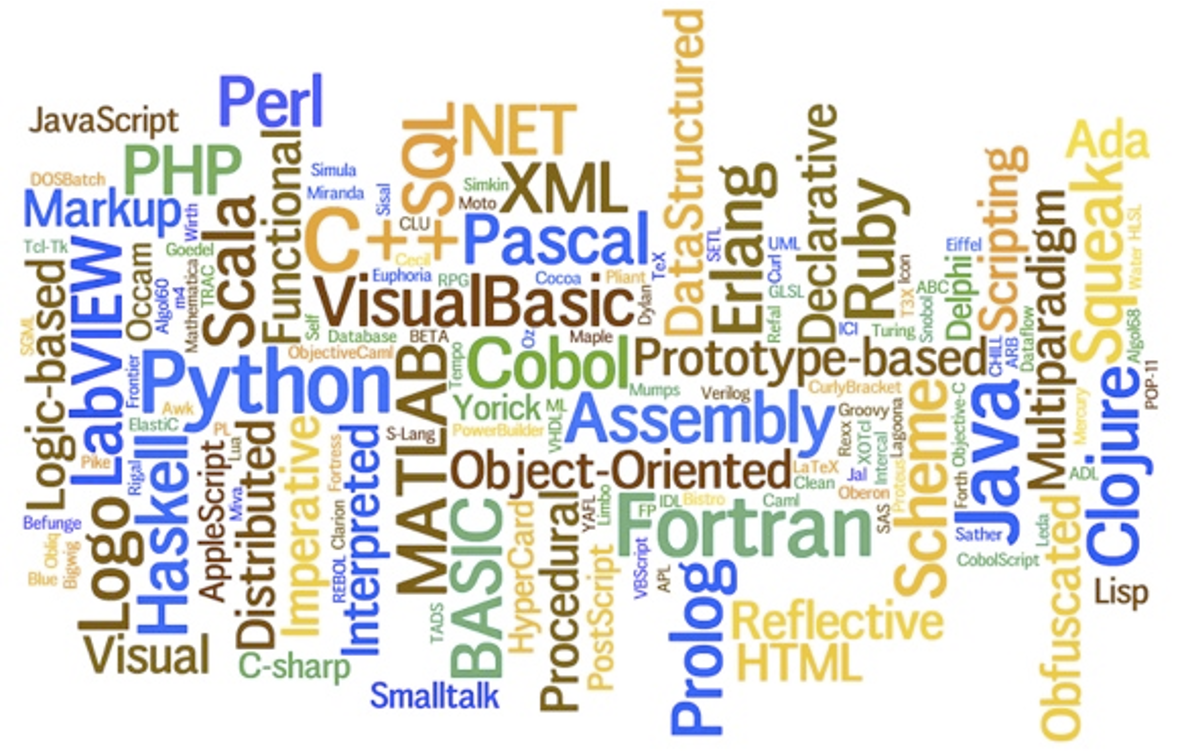
\includegraphics[width=0.6\linewidth]{lectures/figures/9_programming_languages.png}
        \end{figure}
    \end{frame}

    \begin{frame}{Pros and Cons of Programming Languages}
        Pros
        \begin{itemize}
            \item Far more powerful than shell.
            \item Popular ones come with extensive libraries that makes complex math and plotting etc. easier.
            \item Usually comes with support tools (compilers, debuggers, IDEs, etc.) that helps reduce bugs, or at the very least, make them easier to find.
            \item Proper use allows the development of extensible packages and libraries
        \end{itemize}

        Cons

        \begin{itemize}
            \item Compiled languages require an additional compilation step.
            \item Additional learning curve
            \item Not all languages are supported on all systems (though this is usually not an issue with the popular ones)

        \end{itemize}

    \end{frame}

    \begin{frame}{Which Programming Language Should I Choose?}
        Short answer – Whichever one you are most comfortable with.\newline
        \newline
        Long answer – Depends on what you need it for.\newline
        \newline
        If performance is critical (e.g., a DFT code), you probably have to go with compiled languages like C and Fortran.
        If speed of development and prototyping outweighs raw performance, interpreted / scripting languages like Python and Perl are generally easier to get into.\newline
        \newline
        For this class, we will exclusively use Python.

    \end{frame}

    \begin{frame}{What is Python?}
        General-purpose, high-level programming language.\newline
        \newline
        Design emphasizes code readability.\newline
        \newline
        Supports multiple programming paradigms (OOP, imperative, functional, procedural).\newline
        \newline
        Dynamically typed, automatic memory management and large standard library.\newline
        \newline
        Available on almost all platforms.

    \end{frame}

    \begin{frame}{Python vs Other Languages}
        \footnotesize
        Java
        \inputminted{java}{code/9_hello_world.java}
        C
        \inputminted{c}{code/9_hello_world.c}
        Python
        \inputminted{python}{code/9_hello_world.py}

    \end{frame}

    \begin{frame}{Scientific Computing with Python}
        \begin{figure}
            \centering
            
\includegraphics[height=0.8cm]{figures/jupyter-logo.png}
            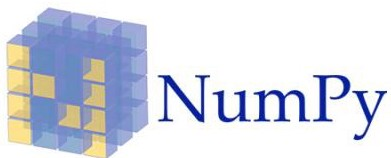
\includegraphics[height=0.8cm]{figures/numpy-logo.jpeg}
            
\includegraphics[height=0.8cm]{figures/scipy-logo.png}
            
\includegraphics[height=0.8cm]{figures/pandas-logo.png}
        \end{figure}
        \begin{description}
            \item[\href{http://jupyter.org/}{jupyter}] Software for interactive computing
            \item[\href{http://www.scipy.org/}{numpy}] Fundamental package for numerical computation. Defines array and matrix types and basic operations on them.
            \item[\href{http://www.scipy.org/}{scipy}] Efficient numerical routines such as routines for numerical integration and optimization.
            \item[\href{http://pandas.pydata.org/}{pandas}] High-performance, easy to use data structures.        \item[\href{http://matplotlib.org/}{matplotlib}] De facto plotting library

        \end{description}
    \end{frame}

    \begin{frame}{Resources}
        \begin{itemize}
            \item \href{https://www.python.org/doc/ }{Python docs}
            \item \href{http://docs.scipy.org/doc/numpy/reference/ }{Numpy docs}
            \item \href{https://docs.jupyter.org/en/latest/start/index.html}{Jupyter docs}
        \end{itemize}
    \end{frame}

    \begin{frame}{Python Libraries for Materials Science}
        \begin{figure}
            \centering
            \begin{subfigure}{0.7\textwidth}
                \centering
                
\includegraphics[width=\linewidth]{lectures/figures/9_pymatgen.png}
                \caption{Python Materials Genomics.\cite{ongPythonMaterialsGenomics2013}}
            \end{subfigure}
            \begin{subfigure}{0.2\textwidth}
                \centering
                
\includegraphics[width=\linewidth]{lectures/figures/9_ASE.png}
                \caption{Atomic Simulation Environment.}
            \end{subfigure}
        \end{figure}
    \end{frame}

    \begin{frame}{Python Materials Genomics (pymatgen)}
        \begin{itemize}
            \item Core materials analysis powering the Materials Project.\cite{ongPythonMaterialsGenomics2013}
            \item Defines core extensible Python objects for materials data representation.
            \item Provides a robust and well-documented set of structure and thermodynamic analysis tools relevant to many applications.
            \item Establishes an open platform for researchers to collaboratively develop sophisticated analyses of materials data.
            \item High-level methods to access the Materials Project API.\cite{ongMaterialsApplicationProgramming2015} (particularly useful for this course).
        \end{itemize}
    \end{frame}


    \begin{frame}{Overview of capabilities}
        \begin{figure}
            \centering
            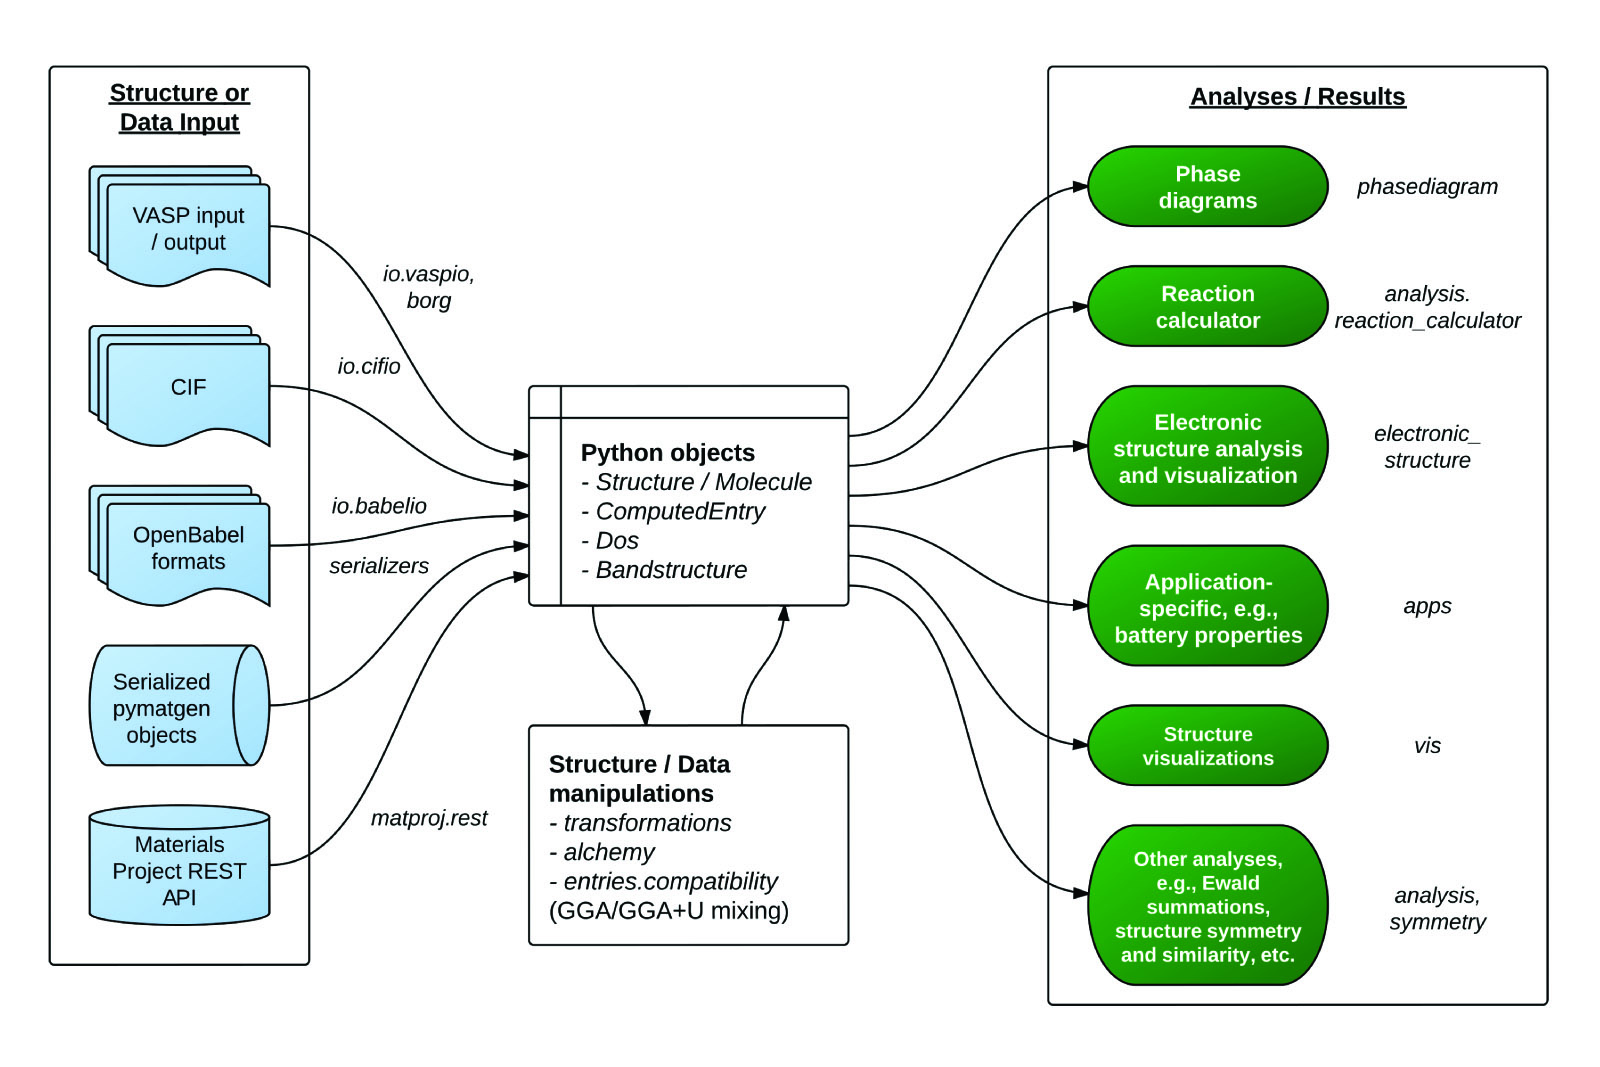
\includegraphics[width=0.6\textwidth]{figures/pymatgen-overview.jpg}
        \end{figure}
    \end{frame}


    \begin{frame}[fragile]{Accessing the Materials API}
        \begin{itemize}
            \item Accessed using the pymatgen.ext.matproj.MPRester class.
            \item Please review the \href{Materials API documentation}{https://api.materialsproject.org}.
            \inputminted{python}{code/example_materials_api.py}
        \end{itemize}
    \end{frame}

    \begin{frame}{Final World on Programming}
        A little investment in learning a programming language can yield big dividends in your efficiency as a materials modeler.
        \begin{figure}
            \centering
            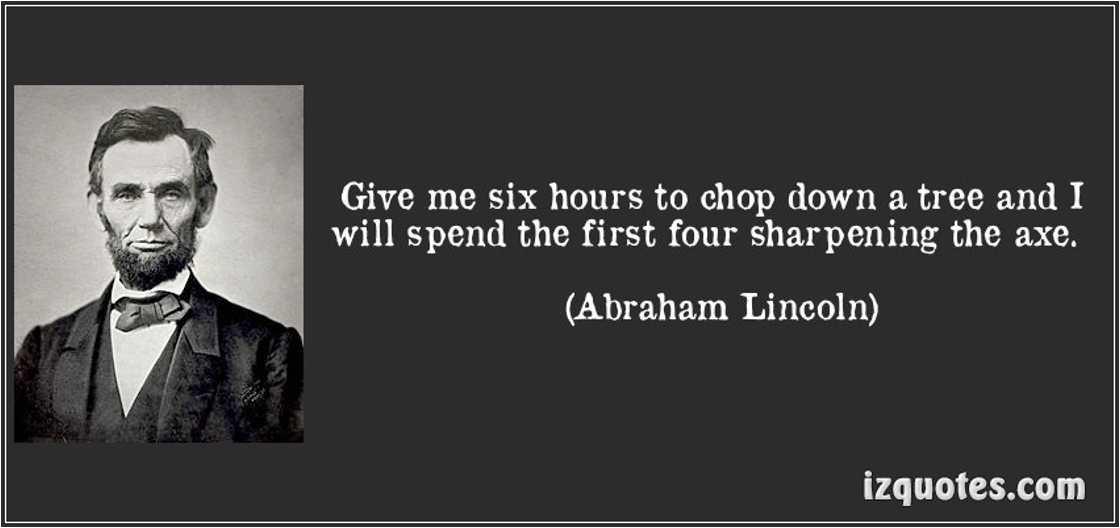
\includegraphics[width=0.7\linewidth]{lectures/figures/9_lincoln.png}
        \end{figure}
    \end{frame}

    \begin{frame}[allowframebreaks]{Bibliography}
        \bibliographystyle{unsrt}
        \bibliography{refs}
    \end{frame}



    \begin{frame}
        \Huge{\centerline{The End}}
    \end{frame}

\end{document}

